\section{The edit method}\label{sec:edit}

The method \code{edit} builds the test from the record itself: it keeps the stretches that carry the
damage, drops the rest, and raises the amplitude only where, and only as much as, the editing could not
keep the damage. It is the practical form of Section~\ref{sec:bzero}. Unlike the methods of Parts~II
and~III it synthesises nothing: the kept stretches are samples of the record, with their waveform,
their spectrum and their sequence of peaks.

\subsection{Windows and their damage shares}\label{sec:editwindows}

The record is cut into $M$ consecutive windows of length $L_w$. The default length is the larger of
2\,s and three amplitude decay times of the slowest oscillator of the grid. The amplitude of a free
response decays as $e^{-\zeta\wn t}$, so its $1/e$ time is $1/(\zeta\wn) = Q/(\pi\fn)$, twice the
response time $\tau$ of~\eqref{eq:tau} (which describes the variance). For $Q = 10$ and $f_{\min} =
5$\,Hz this gives $3\times 0.64 = 1.9$\,s, hence 2\,s; for $Q = 20$ it gives 3.8\,s. A window must be
long enough for the response that a burst excites to lie mostly inside it, otherwise the damage of the
burst is attributed to the next window; it must be short enough to separate the bursts from the quiet
time, otherwise the Lorenz curve flattens. Within these bounds the result depends little on $L_w$.

For every oscillator $i$ the response to the (pre-filtered, Section~\ref{sec:practice}) record is
computed once, cut into the windows, and the rainflow damage of each window is divided by the damage of
the whole record. This gives the matrix of shares $W_{ij}$ of Section~\ref{sec:lorenz}. The damage of
a window computed alone differs slightly from its contribution to the rainflow count of the whole
response, because cycles that span a window boundary are closed differently; the shares are used to
rank and to estimate, the final FDS is always measured on the assembled signal.

\subsection{Ranking the windows}\label{sec:ranking}

Two rankings are available.

\emph{Common.} Windows are sorted by the sum of their shares over the oscillators, $\sum_i W_{ij}$.
This keeps the largest damage on average and is the default.

\emph{Fair.} Windows are added one at a time; each step adds the window that most raises the retention
of the currently worst-served oscillator, $\min_i\sum_{j\in\text{kept}} W_{ij}$ (greedy max--min).
This equalises the retention over the oscillators when different bands want different windows (shocks
at low $\fn$, stationary content at high $\fn$), at the price of a lower average. On the records tested
the fair ranking raised the Lorenz curve of the worst oscillator visibly but did not raise the damage
of the assembled test, because where the damage is spread uniformly in time no ranking can help; the
common ranking remains the default and the fair one an option.

\subsection{Assembly: ring-down margin, cross-fades, time budget}\label{sec:assembly}

The windows are taken in ranking order until the time budget $T/\alpha$ is used. Every kept window is
extended by a ring-down margin of two amplitude decay times $2Q/(\pi f_{\min})$ of the slowest
oscillator, so that the free response excited by a burst at the end of a window stays with the burst
instead of being cut (a window that ends on a shock would otherwise keep the shock and lose the large
cycles of its ring-down). Overlapping stretches are merged; when the next stretch would exceed the
budget the selection stops, and single windows that still fit are added. The stretches are then joined
in their original time order with raised-cosine cross-fades of 0.1\,s (the fades overlap, and the
budget accounts for the overlap). Keeping the original order keeps the slow trends of the record;
a test of duration $T/\alpha$ therefore looks like the record with its quiet parts removed, which is what
it is.

The realised compression differs slightly from the requested one (the budget is used in whole
windows); it is reported. If the requested duration is not shorter than the record, the record is
returned unchanged (with a warning when it is longer).

\subsection{Life and repetitions}

As for the other methods, a life $\Tl$ longer than the record is covered by playing the test $r$ times
(Section~\ref{sec:fds}, with $r$ the rounded ratio $\Tl/T$ of the target). The spectral gain of the
next subsection then aims at the target FDS divided by $r$: the editing compresses the record, the
repetitions cover the life, and the amplitude only makes up for the damage that the editing dropped.

\subsection{Beyond the limit: the spectral gain}\label{sec:gain}

If the requested compression is below the limit~\eqref{eq:alphamax}, the assembled signal already
carries the target damage at every oscillator to within a few percent and the method stops. Beyond the
limit it is missing damage at some oscillators, typically those whose damage was spread uniformly in
time. Raising the whole signal by one factor would also raise the oscillators that lost nothing. The
program therefore applies a frequency-dependent gain $g(f)$, interpolated in $\log f$ between the
nodes, as a zero-phase filter (multiplication of the Fourier transform, so no phase shift and no change
of the peak sequence).

The damage at a node scales as the $b$-th power of the gain in its band (Section~\ref{sec:closedloop}:
$D\propto\sigma_z^b$ and $\sigma_z\propto g$). Writing $r_i = D_i/D_i^{\mathrm{target}}$ for the measured
ratio after a step, the gain of node $i$ is updated as
\begin{equation}\label{eq:gainstep}
  \ln g_i \leftarrow \ln g_i - \frac{\omega_i}{b}\ln r_i ,
\end{equation}
with a relaxation $\omega_i$ that starts at 0.8 and is halved for a node whose error changes sign
between two steps (so that two coupled nodes settle instead of oscillating), a cap of $\pm0.15$ on the
step in $\ln g$, and a clip of $g$ to $[1/g_{\max}, g_{\max}]$ (default $g_{\max} = 2$). Each step
measures the exact rainflow FDS of the gained signal; the loop stops when every node is within the
tolerance (default 5\,\%) or after the step budget. This is the closed loop of
Section~\ref{sec:closedloop} with a gain instead of a PSD.

Two oscillators that are driven by the same input band cannot be set independently by any smooth
gain. The usual case is the top of the grid above the last strong peak of the record: the responses of
the nodes just above the peak are fed by the peak, not by their own band, and a gain between them
raises both. The loop then ends in a compromise, the result table shows the two nodes off the target,
and the program warns when the gain reaches its cap. The remedy is to end the grid where the record
has content, or to accept the compromise.

\begin{result}[What the gain does to the exponent dependence]
After the gain the test is exact at the design exponent $b$ at every node. At another exponent $b'$ the
damage of a node is off by the factor $g_i^{\,b'-b}$ times the (small) factor the editing itself
produces. Where the editing kept the damage, $g_i\approx1$ and the test is right for every exponent;
where the amplitude did the work, the dependence on the exponent is exactly that of an amplitude
scaling. In a plot of $\ln(D_{\mathrm{test}}/D_{\mathrm{record}})$ against $b$ the curves are straight
lines, and their slope $\ln g_{\mathrm{eff}}$ measures how much a test relies on amplitude
(Figure~\ref{fig:exponent}).
\end{result}

\begin{figure}[htb]\centering
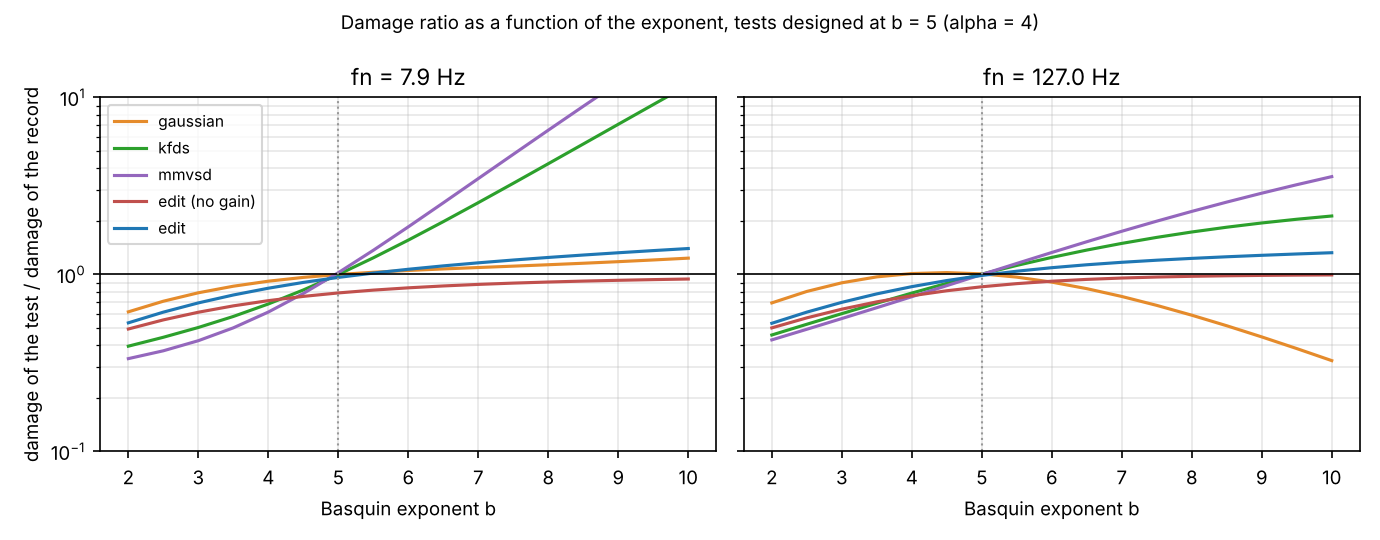
\includegraphics[width=\textwidth]{figures/exponent_example_road.png}
\caption{Example record compressed four times, tests designed at $b = 5$, $Q = 10$: damage of the test
over damage of the record as a function of the exponent at two oscillators. Every synthesis method
crosses 1 at the design exponent and departs from it as a power of its effective amplitude factor; the
edited record without gain stays near 1 for $b\ge5$ (and below 1 at small $b$, the small cycles it
dropped); with the gain it is exact at $b = 5$ and inherits a mild slope where the gain acted.}
\label{fig:exponent}
\end{figure}

\subsection{Results}\label{sec:editresults}

Table~13.1 gives the benchmark of \code{tools/compression\_benchmark.py} on the example record and on
the thesis reference record (the profile of Fig.~3.11 of the dissertation, used in the benchmarks of the
README; the record itself is not distributed):
compression $\alpha = 4$, 17 oscillators from 5 to 200\,Hz at 1/3 octave, $Q = 10$, design $b = 5$,
seed 1. The entries are the geometric mean over the oscillators of the ratio ``damage of the test /
damage of the record'' at each exponent, and in brackets the ratio of the largest to the smallest
value over the oscillators (1 would mean the same ratio at every node).

\begin{center}\small\setlength{\tabcolsep}{4pt}
\begin{tabular}{p{0.26\textwidth}lcccc}
\toprule
Record & Method & $b = 3$ & $b = 5$ (design) & $b = 7$ & $b = 9$ \\
\midrule
example, $\kappa = 6.0$, limit $\alpha_{\max} = 3.0$
 & \code{gaussian} & 0.92 (1.4) & 1.00 (1.1) & 0.74 (1.9) & 0.48 (4.0) \\
 & \code{kfds}     & 0.56 (1.4) & 1.00 (1.1) & 1.77 (2.0) & 2.96 (4.8) \\
 & \code{mmvsd}    & 0.59 (1.7) & 0.99 (1.1) & 1.58 (3.0) & 2.40 (9.0) \\
 & \code{edit}, no gain & 0.65 (1.2) & 0.87 (1.2) & 0.96 (1.1) & 0.98 (1.1) \\
 & \code{edit}     & 0.71 (1.1) & 0.99 (1.0) & 1.15 (1.1) & 1.25 (1.2) \\
\midrule
thesis record, $\kappa = 6.5$, limit $\alpha_{\max} = 1.6$
 & \code{gaussian} & 1.49 (3.6) & 1.00 (4.1) & 0.46 (8.5) & 0.19 (29) \\
 & \code{kfds}     & 0.98 (3.7) & 1.01 (4.3) & 0.87 (11) & 0.74 (82) \\
 & \code{mmvsd}    & 0.63 (1.8) & 0.95 (1.4) & 1.18 (3.5) & 1.34 (13) \\
 & \code{edit}, no gain & 0.52 (2.7) & 0.72 (3.0) & 0.82 (2.9) & 0.86 (2.7) \\
 & \code{edit}     & 0.64 (1.5) & 1.00 (1.1) & 1.29 (1.7) & 1.55 (2.8) \\
\bottomrule
\end{tabular}
\end{center}

\noindent\emph{Table 13.1: damage ratio test/record at four exponents for tests designed at $b = 5$,
$\alpha = 4$.}

Reading the table. At the design exponent every FDS method is right, by construction; the other
columns separate them. On the example record, where the compression is only a little beyond the limit,
the edited record keeps 87\,\% of the damage at $b = 5$ and 98\,\% at $b = 9$ with the same ratio at
every oscillator; the gain adds the missing 13\,\% and a slope of $1.25$ at $b = 9$. The synthesis
methods give half of the damage ($\kappa_z\approx3$ everywhere, the large cycles are missing) or two
to three times the damage at $b = 9$ (the kurtosis they prescribe forces a heavier tail than the
record has, Section~\ref{sec:compressedk}). On the thesis record, whose damage below 100\,Hz is carried
by a few shocks while a stationary band around 160\,Hz dominates the energy, the compression $\alpha =
4$ is well beyond the limit $1.6$: the edited record keeps 72\,\% at $b = 5$, the gain works with factors
up to 1.3 in the stationary band, and the $b = 9$ ratio is 1.55 with a spread of 2.8; the synthesis
methods have spreads of 13 to 82, that is, oscillators where the test is off by one or two orders of
magnitude when the exponent changes, mostly at the top of the grid where the record has little content
of its own. The edited record without gain is the only profile whose ratio has the same order at every
oscillator and every exponent; it is also the only one that is short of the target rather than
beyond it.

Two further observations from the same study. First, the response kurtosis $\kappa_z$ of the edited
test is lower than the record's at the oscillators where quiet time was removed (Section~\ref{sec:compressedk});
MMVSD, which prescribes $\kappa_z$, matches it best, as designed. Second, on a nonlinear oscillator
(a hardening spring, cubic term equal to half the linear one at three times the RMS response) the
edited record transferred the damage with a fidelity of 0.75 to 1.0 relative to its linear fidelity on
both records, while the synthesis methods ranged from 0.35 to 2.7, in both directions depending on the
record: a synthesised signal matches the linear statistics it was designed for, an edited record
carries the waveform. This is one toy nonlinearity and should be read as an indication.
